\chapter{Methods}
In order to prove the hypothesis, a small program to blur images was written. The kind of program was not important, but it was necessary for it to take a significant amount of time and make a measurable impact on the CPU.
The program was benchmarked using profilers. The profiler data shows where delays in the code are located and which language is faster at executing the same procedure. This information allows us to conclude which language, for the purpose of image processing in the form of a Gaussian blur, is more efficient and therefore more environmentally friendly.

\section{Hardware}
Most of the experiments were performed on an Apple MacBook Pro with a 1.4 GHz Quad-Core Intel Core i5 processor. The computer had 16 GB of RAM and 251 GB of flash storage. It was running version 12.3.1 of the MacOS Monterey operating system.

\section{Profilers}
A profiler is a benchmarking tool. It measures the runtime of a program, and other statistics, depending on the profiler. To benchmark our Python program on macOS, a combination of xctrace and cPython was used. For the C++ code on macOS, xctrace was exclusively used.

\subsection{\textit{time}}
At first, the macOS \textit{time} command was used to measure the runtime of the Python program, as seen in figure 6.1.

\begin{figure}[htbp]
	\centering
	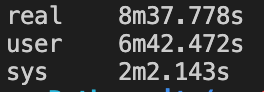
\includegraphics[scale=0.72]{time.png}
	\caption{An example of the \textit{time} command}
	\label{figure:time}
\end{figure}

\textit{time} is a macOS shell keyword that measures the total time spent running the program. The user row shows the time spent in the CPU in user mode, meaning “it does not have direct access to hardware or reference memory and must rely on APIs of the system for delegation. This is how most code runs on your system, and due to its isolation, crashes are always recoverable” \cite{time}. sys stands for system mode or kernel mode. Kernel mode is “when code being executed has unrestricted access to the system hardware” \cite{time}. The first row, called real, is the total time spent in the two modes.

\subsection{XCode Instruments}
In order to keep the research controlled, it was decided to use the same profiler for both programs; Xcode instruments. Xcode is Apple’s IDE and contains Instruments amongst other developer tools. “The Instruments app, which is included with Xcode, gathers data from your running app and presents it in a graphical timeline. With Instruments, one can gather data about performance areas such as our app’s memory usage, disk activity, network activity, and graphics operations” \cite{instruments}. The command-line tool for Instruments is called xctrace, and it is used to record, import, export and symbolicate Instruments .trace files. These .trace files can then be opened in the Instruments app and analysed with the graphical user interface. The CPU Counter template was used most. It was used to track how much time was spent on each part of the program; the algorithm, disk input, disk output and retrieving file names.

\subsection{cProfile}
cProfile is a profiler that is included in the Python standard library. It is a C extension with a reasonable overhead which makes it suitable for profiling long-running programs. It was based on lsprof and contributed by Brett Rosen and Ted Czotter \cite{cprofile}. cProfile measures the total time the program runs, the number of function calls, and the runtime and function calls of each individual function. The measured statistics can be displayed in the command-line interface or a text file.

\section{Energy benchmarking}
The energy used by the programs can be measured by using the Intel® Power Gadget. It is a software-based power usage monitoring tool enabled for Intel® Core™ processors. It is supported on Windows and macOS and includes an application, driver, and libraries to monitor and estimate real-time processor package power information in watts using the energy counters in the processor \cite{powergadget}. The command-line tool PowerLog allows us to measure the energy usage of a program and write it to a log file. Specifically, the log file will include the elapsed time, package power limit, processor frequency, GT (Energy of the processor graphics) frequency, processor temperature, and average and cumulative power of the processor.

\section{Code}
The experiment uses the same algorithm in both languages: Gaussian Blur. In image processing, a Gaussian blur is a result of blurring an image by a two-dimensional Gaussian function which was named after mathematician and scientist Carl Friedrich Gauss. Applying the algorithm to the image causes a blurring effect on the image, the intensity of the blur effect depending on variables like the kernel and standard deviation. The code for the two languages was written to execute as similar as possible.

\subsection{Python}

\begin{listing}[!ht]
\begin{minted}[xleftmargin=20pt, linenos]{python}
#!/usr/bin/env python

import cv2 as cv
import os
import cProfile

pr = cProfile.Profile()
pr.enable()

img_names = os.listdir("/Volumes/RAMDisk/raw")

for name in img_names:
  path = "/Volumes/RAMDisk/raw/{}".format(name)

  if ".DS_Store" in path:4
    continue

  img = cv.imread(path)
  blur = cv.blur(img,(5,5))

  cv.imwrite("/Volumes/RAMDisk/python_blurred/blurred_" + name, blur)

pr.disable()
pr.print_stats()
\end{minted}
\caption{The Python program}
\label{listing:python}
\end{listing}

Looking at listing 1, os is a module that provides a portable way of using operating system dependent functionality \cite{os}. It is used in line 10 to list all image names in the raw images directory. In line 12, a for loop is used to iterate through that list of names, therefore every picture can be blurred, one at a time. Every picture first is “read” in line 18, after determining the path in line 13 and dismissing a possible macOS bug in case the file “.DS\_Store” exists in the directory in lines 15 and 16. In line 19, the Gaussian blur filter is applied to the image using the OpenCV function with parameters of the image variable and Gaussian kernel size. Line 21 shows the blurred image being written to the disk.
In listing 1, the profiler cProfile being used. It is imported in line 5 and initialised in line 7. Line 8 enables the profiler and line 23 disables it so it is wrapped around the code we want to profile. In line 24 the collected statistics are printed to the console or a file.

\subsection{C++}

\begin{listing}[!ht]
\begin{minted}[xleftmargin=20pt, linenos]{c++}
#include <opencv2/opencv.hpp>
#include <iostream>
#include <string>
#include <filesystem>
#include <vector>

using namespace cv;
using namespace std;

namespace fs = std::__fs::filesystem;
\end{minted}
\caption{The C++ program requirements}
\label{listing:c++requirements}
\end{listing}

Listing 2 shows the beginning of the C++ code. First, the OpenCV and C++ standard libraries are imported and the namespaces are assigned.

\begin{listing}[ht]
\begin{minted}[xleftmargin=20pt, linenos]{c++}
int main(int argc, char* argv[])
{
  if (argc < 3) {
    cout << "Usage: ./green_apple_blur <input_path> <output_path>" << endl;
    return 1;
  }

  string base_path = argv[1];
  string ds = ".DS_Store";

  for (const auto & file : std::__fs::filesystem::directory_iterator(base_path))
  {
    fs::path path = file.path();
    string filename = path.filename().string();

    if (find(path.begin(),path.end(),ds)!=path.end())
      {
        continue;
      }

\end{minted}
\caption{Reading the image file}
\label{listing:c++-read}
\end{listing}

In listing 3, the path to the images is added as a parameter to the main function when the program is run in line 1. To prevent a bug the file “.DS\_Store” in the path in line 16 is ignored.

\begin{listing}[ht]
\begin{minted}[xleftmargin=20pt, linenos]{c++}

    // Read the image file
    Mat image = imread(path);

    // Check for failure
    if (image.empty())
      {
        cout << "Could not open or find the image" << endl;
        cin.get(); //wait for any key press
        return -1;
      }

    //Blur the image with 5x5 Gaussian kernel
    Mat image_blurred;
    GaussianBlur(image, image_blurred, Size(5, 5), 0);

    string writePath = argv[2];

    string blur_path = writePath + "/blurred_" + filename;
    bool isSuccess = imwrite(blur_path, image_blurred); //write the image to a file as JPEG

    if (isSuccess == false)
      {
        cout << "Failed to save the image" << endl;
        cin.get(); //wait for a key press
        return -1;
      }
    }

    return 0;
}
\end{minted}
\caption{Processing and writing the image file to the disk}
\label{listing:c++-write}
\end{listing}

In line 2 of listing 4, the image file is read with the OpenCV imread function. In line 14 the image is blurred with the GaussianBlur filter function from OpenCV \cite{gaussianblur}. Size (5, 5) is the Gaussian kernel size, it should be an odd number. The last zero controls the sigma value which is the standard deviation in the X direction and the Y direction of the Gaussian distribution. It will be calculated based on the size of the kernel \cite{gaussianblurtutorial}. In line 19 the image is saved to the path specified in the parameter and the success of that operation is checked. At the end, 0 is returned to terminate the function successfully.
